
\chapter{Units, Physical Quantities, and Vectors}

\section{Notes}

The most important thing about this section is 
\begin{itemize}
	\item{Using the units to ensure that calculation are correctly performed.}
	\item{Estimating results to determine get a good feel on if your result makes sense.}
	\item{Error notation and their meaning. Mostly just to understand what you are reading.}
\end{itemize}

Understanding vectors is nice, but you should not spend more than a few minutes reading about them. In most cases you can "learn on the job". The only important things you need to know right now are,

\begin{itemize}
	\item{Vectors have a direction and a magnitude (length).}
	\item{Vectors are made of components; usually x, y, and z in Physics.}
	\item{In most cases vector components are independent of the component. For example, Up/Down don't impact left/right.}
\end{itemize}

\section{Discussion Questions}

% 1.1
\discussion{We just need a single experiment to disprove a theory.  However, there is no number of experiments to prove a theory, just increase confidence.  If there are only a finite number of possible outcomes this is obviously not true..}

% 1.2
\discussion{Two possible answers based on what they mean by tangent, 1) The tangent function takes in degrees and not distances. 2) The tangent of a line requires a function (or a continuous set of points) to compute a the tangent of a line.}

% 1.3
\discussion{My height in imperial is 6' 2", which is 187.96 cm.  My weight is 178 lbs in imperial and therefore it is 792.1 N}

% 1.4
\discussion{Yes.  Currently the mass is derived directly from these.  Other quantities are based off of properties events in nature, but the mass is derived by humans. As an aside, the mass increase is probably from oxidation or some similar process in which the reference mass is absorbing molecules or elements from the air.}

% 1.5
\discussion{You could use pulsars as a way to measure time as they have a very precise rotation.  Less precise measures could be position of sun in the sky to determine the hour of day.}

% 1.6
\discussion{Let's assume an 8 by 11 inch sheet of paper.  Then you can cut it into squares of 1x1 inch and then stack them up.  Measure that value and then divide it by 88 to approximate the thickness of a piece of paper. An alternative is to just fold it instead of cutting it up, but then you will not be able to get a more accurate answer.}

% 1.7
\discussion{An axiom is a self consistent statement.  It does not mean that it matches reality.  In terms of physics you could argue that an axiom is only true if the assumptions you are making are true.  A theory is only true as far as the experiments have shown it to be the best match based on observations.}

% 1.8
\discussion{The units of volume are meter-cubed and centimeter-cubed. The provided formula is "length" to the fourth, not the third as required.}

% 1.9
\discussion{Joe is not accurate but is precise, Moe is accurate but not precise, Flo is both accurate and precise.}

% 1.10
\discussion{No, the length of $(1,1,1)$ is $\sqrt{3}$.  No, the length of $(3,-2)$ is $\sqrt{11}$}

% 1.11
\discussion{Simple math, $\frac{9.8*60}{0.03^2} \approx{} 653KN/m$, $\frac{9.8*600}{0.092903} \approx{} 63KN/m$, over a 10x difference.}

% 1.12
\discussion{There are no two vectors with different lengths that when summed together are 0.  This is due to the fact of dimensional independence requires that to get 0 the entries in the vector as the same position must have the same magnitude but different sign.  To get three vectors of different lengths you can create three vectors of the form: $\vec{A} = (x,y,0), \vec{B} = (-x,0,z), \vec{C} = (0,-y,-z)$ where $|x| > |y| > |z|$. From here it is easy to show that $|\vec{A}| > |\vec{B}| > |\vec{C}|$.}

% 1.13
\discussion{The speed of light is 299,792,458 m/s and the radius of the earth is 6,400 km, or 6,400,000 m.  Therefore the circumference, 2$\pi{}$r, is 40,212,385.9659, then the circumference divided by the speed of light is 0.1341340814 seconds.}

% 1.14
\discussion{These are not vectors as they have no distance.}

% 1.15
\discussion{Only if dealing with imaginary numbers. Otherwise you will have a magnitude of $\sqrt{A^2 + B^2}$ and the only way that is zero is if A and B are both zero.  As before this would have to involve imaginary numbers.  You can do a proof to show that $\sqrt{\sum A_i^2} \geq |A_i| \forall i$}

% 1.16
\discussion{(a) No. (b) Only in reference to another vector, which points in the opposite direction.  Because all the component values of the two vectors are negatives of each other.  i.e $\vec{A}$ is the negative of $\vec{B}$ if-and-only-if $\forall i~A_i = -B_i$}

% 1.17
\discussion{For the first question $\vec{A}$ and $\vec{B}$ are multiples if each other. For the second question they both have to be the zero vector.}

% 1.18
\discussion{No.  Since neither are the zero vector when using the formulas $|\vec{A}| |\vec{B}| \cos{\alpha}$ and $|\vec{A} \times{} \vec{B}| = |\vec{A}||\vec{B}|\sin{\alpha}$ either $\sin{\alpha}$ or $\cos{\alpha}$ is 0 but not both.}

% 1.19
\discussion{No.  Time has a single component, and you can also do a 1:1 mapping to the reals (trivially) which is defined to be a scalar.}

% 1.20
\discussion{You can work out the math to show it is a unit vector, the direction is the same direction as $\vec{A}$.  Using the identify $\vec{A}/A \cdot \vec{i} = |\vec{A}/A||\vec{i}|cos{\left(\alpha\right)}$ then we have the right side just equal to $cos{\left(\alpha\right)}$.}

% 1.21
\discussion{The percent error is $1 - \frac{890010}{890000} = 1\mathrm{e}{-6}\%$.  You can argue in this case it is correct to display all digits as the exact distances are known.}

% 1.22
\discussion{Assuming 3-dim vectors, (a) Valid (b) Valid (c) Valid (d) Valid (e) No, cannot do cross product between Vector and scalar.}

% 1.23
\discussion{The cross product products a vector which is orthogonal to the original as long as not same vector.  You can just pick $\vec{A}$ and $\vec{B}$ to be the same.  If they are all zero obviously they are same.}

% 1.24
\discussion{Cross product produces vector orthogonal to original two.  The dot product of two orthogonal vectors is 0.}

% 1.25
\discussion{No.  $\vec{A} = (1,0,0)$ and $\vec{B} = (0,1,0)$ will satisfy this.}

% 1.26
% TODO : Figure out what they are asking.
\discussion{I don't know what they are talking about.  Their question makes no sense.}

\section{Exercises}

\subsection{Standard and Units, Using and Converting Units}

% 1.1
\exercise{ Some definitions: 1in = 2.54cm, 12in = 1ft, 5280ft = 1 mi, 2.54 * 5280 * 12 / 100000 = (a) 1.60 mi = 1.60 mi * 5280ft/mi =  2.57 km (b) 1.18 miles}

% 1.2
\exercise{28.9 in$^3$}

% 1.3
\exercise{$5.59\mathrm{e}{-9}$}

% 1.4
\exercise{13.5 g/cm$^3$ $\to$ 13.5$\mathrm{e}{3}$ kg/m$^3$ }

% 1.5
\exercise{5.36 L}

% 1.6
\exercise{6.86 Hectares}

% 1.7
\exercise{34.9 Years older}

% 1.8
\exercise{185000 furlong/fortnight $\cdot$ $\frac{1}{8}$ mi/furlong $\cdot$ $\frac{1}{14}$ fortnight/days $\cdot$ $\frac{1}{24}$ day/hour = 66.96428571 mi/hour $\approx$ 67.0 mi/hour.}

% 1.9
\exercise{(a) 23 \si{\kilo\meter/\liter} (b) 1.6 Tanks}

% 1.10
\exercise{(a) 88 ft/s (b) 9.754 \si{\meter/\second^2} (c) 1000 $\si{\kilo\gram/\meter^3}$}

% 1.11
\exercise{9.0 \si{\centi\meter}}

% 1.12
\exercise{(a) 4.10$\times$10$^8$ \si{\micro\gram/day}}

% 1.13
\exercise{(i) $\frac{32}{3}\times10^{-8}$ (ii) $8\pi\times10^{-6}\si{\milli\meter^2}$}

\subsection{Uncertainty and Significant Figures}

% 1.14
\exercise{(a) \num{96} \si{\milli\meter^2} (b) 0.37 (c) 43.96 \si{\milli\meter} (d) 10 \si{\milli\meter} (e) 2.7}

% 1.15
\exercise{$\approx{0.45\%}$}

% 1.16
\exercise{(a) 3.14236 (b) 3.14159 (c) a: No, b: Yes}

\subsection{Estimates and Orders of Magnitude}

% 1.17
\exercise{Height in \si{\centi\meter}}

% 1.18
\exercise{16,000}

% 1.19
\exercise{7.1 $\times$ $10^8$ blinks in a lifetime}

% 1.20
\exercise{(a) 17 $\times$ $10^3$ \si{\meter^3/year} (b) 32 \si{\meter}}

% 1.21
\exercise{Average height of a female is 161.8 \si{\centi\meter} tall, assume $\approx{30 \si{\centi\meter}}$ wide and assume wall is 1 \si{\centi\meter} thick.  $\approx{\$936,000}$.}

% 1.22
\exercise{Estimations: beats/min$\approx{90}$, lifetime$\approx{80 years}$ (a) 3.8 $\times$ $10^9$ beats in a lifetime. (b) 5.0 $\times$ $10^7$ gallons pumped in a lifetime.}

% 1.23
\exercise{Estimations: diameter$\approx{1 \si{\milli\meter}}$ 2.4 $\times$ $10^5$ drops in a bottle}

\subsection{Vectors and Vector Addition}

\begin{figure}[!ht]
    \centering
\begin{tikzpicture}[scale=0.1]
  \coordinate (origo) at (0,0);

  % Sheet  
  \draw[thin,gray!40] (-17,-17) (17,17);
  \draw[->] (0,0)--(-17,0) node (-x) [left]{};
  \draw[->] (0,0)--(17,0) node (x) [right]{$x$};
  \draw[<->] (0,-17)--(0,17) node (y) [above]{$y$};
  
  % Vectors
  \draw[blue,->,thick] (0,0) -- (70:15) %
  	coordinate (B) node[right, text width=5em] %
  	{$\boldsymbol{\vec{B} (15 \si{\meter})}$};
  	
  \draw[blue,->,thick] (0,0) -- (143:10) %
  	coordinate (D) node[left, text width=5em] %
  	{$\boldsymbol{\vec{D} (10 \si{\meter})}$};
  	
  \draw[blue,->,thick] (0,0) -- (205:12) %
	coordinate (C) node[left, text width=5em] %
  	{$\boldsymbol{\vec{C} (12 \si{\meter})}$};
  	
  \draw[blue,->,thick] (0,0) -- (270:8) %
  	coordinate (A) node[right, text width=5em] %
  	{$\boldsymbol{\vec{A} (8 \si{\meter})}$};
  	
  % Angles
  \pic %
  	[
  		draw,
  		<-,
  		"$\ang{30.0}$"scale=0.75,
  		angle eccentricity=1.5,
  		angle radius=1cm
  	] %
  	{angle = B--origo--y};
  	
  \pic %
  	[
  		draw,
  		<-,
  		"$\ang{53.0}$"scale=0.75,
  		angle eccentricity=1.5,
  		angle radius=0.5cm
  	] %
  	{angle = y--origo--D};
  	
  \pic %
  	[
  		draw,
  		<-,
  		"$\ang{25.0}$"scale=0.75,
  		angle eccentricity=1.5,
  		angle radius=0.75cm
  	] %
  	{angle = -x--origo--C};
\end{tikzpicture}
    \caption{Problem 1.24}
    \label{fig:Problem1.24}
\end{figure}

% 1.24
\exercise{Using \Fig{fig:Problem1.24}.  Doing this in my head. (a) Angle, maybe around \ang{30} (\ang{33}), Looks around 10\si{\meter} (9\si{\meter}) (b) Angle, maybe \ang{25} (\ang{20}) from the negative y-axis and probably 20 m (c) Same as a but angle is now from negative x-axis (d) Same as b but angle is now from positive y-axis.}

% 1.25
\exercise{Magnitude: 7.83 \si{\kilo\meter}, Angle: \ang{38}}

% 1.26
\exercise{$(230,-37)$ \si{\meter}, Mag: 230 \si{\meter}, Deg: \ang{350}}

\subsection{Components of Vectors}

% 1.27
\exercise{Using \Fig{fig:Problem1.24}. \\
\mbox{} \\
\begin{tabular}{l l l l l}
Vector & Magnitude & Angle & X & Y \\ \hline
A & 270 \si{\meter} & \ang{8}  &  0 \si{\meter}    & -8 \si{\meter}    \\
B & 60 \si{\meter}  & \ang{15} &  7.5  \si{\meter} &  13.0 \si{\meter} \\
C & 205 \si{\meter} & \ang{12} & -10.9 \si{\meter} & -5.07 \si{\meter} \\
D & 143 \si{\meter} & \ang{10} & -7.99 \si{\meter} &  6.02 \si{\meter}
\end{tabular}}

% 1.28
\exercise{(a) \ang{335} (b) \ang{20.7} (c) \ang{122} (d) \ang{226} }

% 1.29
\exercise{
\begin{tabular}{l l l l l}
	x     & y  & angle & mag \\ \hline
	-8.12 \si{\meter} & 13 \si{\meter} & \ang{122}   & 15.3 \si{\meter}
\end{tabular}
}

% 1.30
\exercise{
\begin{tabular}{l l l l}
	x     & y   & angle & mag \\ \hline
	-20 \si{\meter}	  & -24 \si{\meter} & \ang{230}	& 31 \si{\meter}
\end{tabular}}

% 1.31
\exercise{
\begin{tabular}{l l l l l}
	Vector & X & Y & Angle & Magnitude \\ \hline
	A+B	&  7.5 \si{\kilo\meter} &  5.00 \si{\kilo\meter} & \ang{33.6} &	9.01 \si{\kilo\meter} \\
	B+A	&  7.5 \si{\kilo\meter} &  5.00 \si{\kilo\meter} & \ang{33.6} &	9.01 \si{\kilo\meter} \\
	B-A	&  7.5 \si{\kilo\meter} &  21.0 \si{\kilo\meter} & \ang{70.3} & 22.3 \si{\kilo\meter} \\
	A-B	& -7.5 \si{\kilo\meter} & -21.0 \si{\kilo\meter} & \ang{70.3} & 22.3 \si{\kilo\meter}
\end{tabular}}

% 1.32
\exercise{Magnitude: 7.83 \si{\kilo\meter}, Angle: \ang{38}}

% 1.33
\exercise{
\begin{tabular}{l l l l}
	x    & y    & angle & mag \\ \hline
	1.95 \si{\kilo\meter} & -3.9  \si{\kilo\meter}& \ang{296} & 4.36 \si{\kilo\meter}
\end{tabular}}

% 1.34
\exercise{
\begin{tabular}{l l l l}
	x    & y    & angle & mag \\ \hline
	-8.60 \si{\centi\meter} &  5.20 \si{\centi\meter} & \ang{329}  & -10.0 \si{\centi\meter} \\
	-9.70 \si{\meter} & -2.45 \si{\meter} & \ang{14.2} & -10.0 \si{\meter} \\
	 7.75 \si{\kilo\meter} & -2.70 \si{\kilo\meter} & \ang{341}  &  8.21 \si{\kilo\meter}
\end{tabular}}


\begin{figure}[!ht]
    \centering
\begin{tikzpicture}[scale=0.7]
  \coordinate (origo) at (0,0);

  % Sheet  
  \draw[thin,gray!40] (-2,-2) (3,3);
  \draw[<->] (-2,0)--(3,0) node (x) [right]{$x$};
  \draw[<->] (0,-2)--(0,3) node (y) [above]{$y$};
  
  % Vectors
  \draw[blue,->,thick] (0,0) -- (60:2.8) %
  	coordinate (A) node[right, text width=5em] %
  	{$\boldsymbol{\vec{A}}~(2.8~\si{\centi\meter})$};%
  \draw[blue,->,thick] (0,0) -- (-60:1.90) %
  	coordinate (B) node[right, text width=5em] %
  	{$\boldsymbol{\vec{B}}~(1.9~\si{\centi\meter})$};%
% Angles
  \pic %
  	[
  		draw,
  		<->,
  		"$\ang{60.0}$"scale=0.75,
  		angle eccentricity=1.5,
  		angle radius=1cm
  	] %
  	{angle = x--origo--A};
  	
  \pic %
  	[
  		draw,
  		<->,
  		"$\ang{60.0}$"scale=0.75,
  		angle eccentricity=1.5,
  		angle radius=1cm
  	] %
  	{angle = B--origo--x};
\end{tikzpicture}
    \caption{Problem 1.35}
    \label{fig:Problem1.35}
\end{figure}


% 1.35
\exercise{Using \Fig{fig:Problem1.35}. \\
\mbox{} \\
\begin{tabular}{l l l l l}
    Vector &  Angle & Magnitude \si{\centi\meter} &  X \si{\centi\meter}   &  Y \si{\centi\meter}	 \\ \hline
    A+B    &  18.3  & 2.48      &  2.35 &  0.779 \\
    A-B    &  83.7  & 4.10      &  0.45 &  4.07  \\
    B-A    &  264   & 4.10      & -0.45 & -4.07
\end{tabular}}

\subsection{Unit Vectors}

% 1.36
\exercise{
\begin{tabular}{l l l}
	Part &  X    & Y     \\ \hline
	a    &  3.20 & -6.50 \\
	b    & -7.91 & 18.2  \\
	c    & -12   & 21.2  \\
	d    &  40   & -20
\end{tabular}}

% 1.37
\exercise{
\begin{tabular}{l l}
	Name & value  \\ \hline
	A    & $(0\hat{i} - 8\hat{j})$ \\
	B    & $(7.5\hat{i} + 13\hat{j})$ \\
	C    & $(-10.9\hat{i} - 5.07\hat{j})$ \\
	D    & $(-7.99\hat{i} + 6.02\hat{j})$
\end{tabular}}

\begin{figure}[!ht]
    \centering
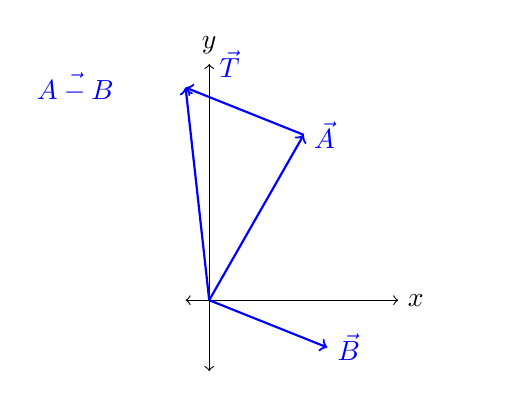
\begin{tikzpicture}[scale=0.3]
  \coordinate (origo) at (0,0);

  % Sheet  
  \draw[thin,gray!40] (-1,-3) (8,10);
  \draw[<->] (-1,0)--(8,0) node (x) [right]{$x$};
  \draw[<->] (0,-3)--(0,10) node (y) [above]{$y$};
  
  % Vectors
  \draw[blue,->,thick] (0,0) -- (4,7) %
  	coordinate (A) node[right, text width=5em] %
  	{$\boldsymbol{\vec{A}}$};%
  \draw[blue,->,thick] (0,0) -- (5,-2) %
  	coordinate (B) node[right, text width=5em] %
  	{$\boldsymbol{\vec{B}}$};%
  \draw[blue,->,thick] (4,7) -- (-1,9) %
  	coordinate (T) node at (0,10) [right, text width=5em] %
  	{$\boldsymbol{\vec{T}}$};%
  \draw[blue,->,thick] (0,0) -- (-1,9) %
  	coordinate (A-B) node[left, text width=5em] %
  	{$\boldsymbol{\vec{A-B}}$};%
\end{tikzpicture}
    \caption{Problem 1.38}
    \label{fig:Problem1.38}
\end{figure}

% 1.38
\exercise{(a) $|\vec{A}| = $8.06 $|\vec{B}|$ = 5.39 (b) -$\hat{i} + 9\hat{j}$ (c) 9.06 \ang{96.3} (d) See \Fig{fig:Problem1.38}.
}


\begin{figure}[!ht]
    \centering
\begin{tikzpicture}[scale=0.7]
  \coordinate (origo) at (0,0);

  % Sheet  
  \draw[thin,gray!40] (-3,-3) (5,4);
  \draw[->] (0,0)--(-3,0) node (-x) [right]{};
  \draw[<->] (0,0)--(5,0) node (x) [right]{$x$};
  \draw[<->] (0,-3)--(0,4) node (y) [above]{$y$};
  
  % Vectors
  \draw[blue,->,thick] (0,0) -- (70:3.6) %
  	coordinate (A) node[right, text width=5em] %
  	{$\boldsymbol{\vec{A}}~3.6 m$};%
  \draw[blue,->,thick] (0,0) -- (210:2.4) %
  	coordinate (B) node[below, text width=5em] %
  	{$\boldsymbol{\vec{B}}~2.4 m$};%
% Angles
  \pic %
  	[
  		draw,
  		<->,
  		"$\ang{70.0}$"scale=0.75,
  		angle eccentricity=1.5,
  		angle radius=1cm
  	] %
  	{angle = x--origo--A};
  	
  \pic %
  	[
  		draw,
  		<->,
  		"$\ang{30.0}$"scale=0.75,
  		angle eccentricity=1.5,
  		angle radius=1cm
  	] %
  	{angle = -x--origo--B};
\end{tikzpicture}
    \caption{Problem 1.39}
    \label{fig:Problem1.39}
\end{figure}

% 1.39
\exercise{\Fig{fig:Problem1.39} as reference.  \\
(a) $\vec{A} = 2.08\hat{i}~\si{\meter} + 1.20\hat{j}~\si{\meter}$, $\vec{B} = -1.23\hat{i}~\si{\meter} - 3.38\hat{j}~\si{\meter}$ \\
(b) $\vec{C} = 11.2\hat{i}~\si{\meter} + 17.1\hat{j}~\si{\meter}$ \\
(c) 20.4~\si{\meter}}

% 1.40
\exercise{(a) \ang{153} (b) \ang{15.9} (c) \ang{63.4}}

% 1.41
\exercise{
(a) $|\vec{A}|=5.39$ $|\vec{B}|=4.369$ \\
(b) $\vec{A}-\vec{B} = -5\hat{i} + 2\hat{j} + 7\hat{k}$ \\
(c) $|\vec{A}-\vec{B}| = 8.83$. Opposite direction but same magnitude.
}

\subsection{Products of Vectors}

% 1.42
\exercise{\ang{82.1}}

% 1.43
\exercise{
(a) 104 (b) -148 (c) -40.6
}

% 1.44
\exercise{$(0,0,-43)$}

% 1.45
\exercise{
(a) \ang{165}
(b) \ang{28.1}
(c) \ang{90}
}

% 1.46
\exercise{ (a) mag: 4.61 dir: $(0,0,-1)$ (b) mag: 4.61 dir: $(0,0,1)$}

% 1.47
\exercise{(a) mag: 64.9 dir: $(0,0,-1)$ (b) mag: 63.9 dir: $(0,0,1)$}

% 1.48
\exercise{(a) -7.47 (b) mag: 4.33 dir: $(0,0,-1)$ }


\section{Problems}

\problem{
Common Stuff:
$Density=\frac{Mass}{Volume}$\\
Volume = $\frac{4}{3}\pi{}r^3$. \\


A) Earth Radius: 6.371*$10^{6}$m, Earth Mass: 5.972*$10^{24}$kg \\
Volume = = $\frac{4}{3}\pi{}(6.371*10^{6})^2$ \\
So the density is $\frac{3* 6.371}{4 * \pi * (5.972)^3} * \frac{10^{24}}{(10^6)^3}$ and Excel says this is equal to $5.51*10^3 kg/m^3$. I doubled checked online and it matches up. To convert to $g/cm^3$ just multiple by 1/1000 to get $5.51~g/cm^3$ \\


B) Sun Mass: $1.989*10^{30}$ \\
Density = $\frac{3 * 1.989}{4 * \pi * 255} * \frac{10^{30}}{10^{8}} = 1.41*10^{17}kg/m^3 = 1.41*10^{14}g/cm^3$. \\


C) Just the same formula for (B) but 20km and you get $1.78*10^{20} kg/m^3$ or $1.78*10^{17}g/cm^3$
}
\section{Challenge Problems}